\documentclass{article}
\usepackage[utf8]{inputenc}
\usepackage{tikz}
\usepackage{verbatim}
\usetikzlibrary{trees,arrows}

\title{TP2-IFT3913}
\author{Wenhao Xu, 20150702\\Manping Li, 968527}
\date{}


\begin{document}

\maketitle

\section*{Tâche 1}

\tikzstyle{level 1}=[level distance=30mm, sibling distance=30mm]
\tikzstyle{level 2}=[level distance=30mm, sibling distance=15mm]
\tikzstyle{level 3}=[level distance=20mm]
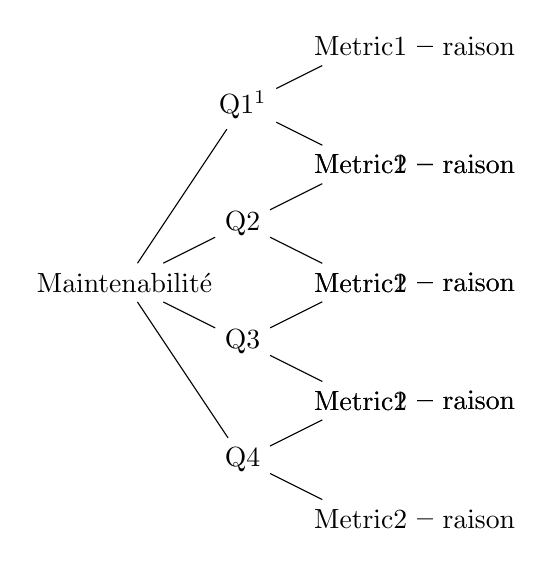
\begin{tikzpicture}[grow=right]
\begin{scope}[yshift=-6cm]
  \node {Maintenabilité}
    child {node {Q4}
      child {node {Metric2}
        child[-] {node{raison}}  
      }
      child {node {Metric1}
        child[-] {node{raison}}  
      }
    }
    child {node {Q3}
      child {node {Metric2}
        child[-] {node{raison}}  
      }
      child {node {Metric1}
        child[-] {node{raison}}  
      }
    }
    child {node {Q2}
      child {node {Metric2}
        child[-] {node{raison}}  
      }
      child {node {Metric1}
        child[-] {node{raison}}  
      }
    }
    child {node {Q1\footnotemark}
      child {node {Metric2}
        child[-] {node{raison}}  
      }
      child {node {Metric1}
        child[-] {node{raison}}  
      }
    };
\end{scope}
\end{tikzpicture}


\footnotetext{Q1 : Le niveau de documentation des classes est-il approprié par rapport à leur complexité?, 
Q2 : La conception est-elle bien modulaire?, Q3 : Le code est-il mature?, Q4 : Le code peut-il être testé 
bien automatiquement?}

\end{document}
